% !TeX root = main.tex
% preamble
\documentclass[11pt,a4paper,twocolumn]{article}
\usepackage[norsk]{babel}
\usepackage[a4paper,
top=2cm,
bottom=2cm,
left=3cm,
right=3cm,
marginparwidth=1.75cm]{geometry}
\usepackage{amsmath}
\usepackage[norsk]{cleveref}
\usepackage[shortlabels]{enumitem}
\usepackage{graphicx}
\usepackage[T1]{fontenc}
\usepackage[hyphens]{url}
\usepackage{lipsum} 
\usepackage{siunitx}

%få tabell og kretser til å vises når man compilerer
\usepackage{float}
\usepackage{tabularx}
\usepackage{caption}

%Venstre justerer alle tabellene slik at de ligger pent langs den delte siden. 
\captionsetup[table]{
	justification=raggedright,
	singlelinecheck=false,
	labelfont=normalfont,
	textfont=normalfont,
	skip=3pt
}

%Figurtekst
\captionsetup[figure]{
	skip=2pt
}

% Lar deg bruke \hl{} for å lage gul markering i teksten
% tiltenkt brukt til å markere seksjoner vi må jobbe mer med.
\usepackage{xcolor}
\usepackage{soul}
\sethlcolor{yellow}

\sisetup{
	output-complex-root = \ensuremath{\mathit{j}},
	complex-root-position = before-number,
	exponent-product = \cdot,
	output-decimal-marker = {,}
}
\usepackage{tikz}
\usepackage{circuitikz}
\usetikzlibrary{arrows.meta,positioning,calc}
\usepackage{pgfplots}
\pgfplotsset{compat=1.18}
\setlength{\parindent}{0pt}

% metadata
\title{Oblig 1. }
\author{Gruppe ADK57\\\\Odin Heggvold Bekkelund\\Caritha Lorenza Furnes\\ Geir Ove VenstadGeir Ove Venstad\\Markus Øfjord }
\date{31.08.2026} 

% definer en url til senere?
\urldef{\myoverleafurl}\url{https://tinyurl.com/2yfbtdez}

% selve dokumentet starter
\begin{document}
	
	\maketitle % Setter sammen \title og \author og \date
	
	\begin{abstract}
	I første del av øvelsen ble det analysert hvordan elektriske kretser kan fungere med bryter ved å undersøke hvordan en bryter fungerer. Deretter ble det laget ulike kretser der målet var analysere hvordan motstand, dioler, bryter og strøm påvirker hverandre. 
	\end{abstract}
	
	% Innholdsfortegnelse automatisk generert:
	%\tableofcontents
	
	\section{Nomenclature}
	\begin{table}[H]
		\caption{Liste over notasjon benyttet for denne øvelsen.}
		\label{tab:notasjon}
		\noindent
		\begin{tabular}{@{}lll@{}}
			\hline
			Størrelse & Symbol & Enhet \\
			\hline
			Spenning & $v$ & V \\
			Strøm & $i$ & A \\
			Motstand & $R$ & $\Omega$ \\
			\hline
		\end{tabular}
	\end{table}
	
	\section{Innledning}
	Formål med øvelsen var å undersøke hvordan ulike komponenter i ulike elektriske kretser påvikrer hverandre. Utstyr som ble benyttet i øvelsen er listet i tabell 2.

\begin{table}[H]
	\caption{Utstyrsliste}
	\label{tab:utstyr}
	
	\small
	\begin{tabularx}{\columnwidth}{@{}lXX@{}}
		\hline
		\textbf{Utstyr} & \textbf{Type} & \textbf{Fabrikat} \\
		\hline
		Breadboard & -- & -- \\
		Ledninger & -- & -- \\
		Diode & Light Emitting & -- \\
		Knapp & Trykk & -- \\
		Multimeter & Digitalt & Elma Instruments \\
		Batteri & \qty{9}{\volt} & Kjell\&Company \\
		Motstand & \qty{200}{\ohm} & -- \\
		\hline
	\end{tabularx}
\end{table}


\section{Teoretisk del}
\subsection{Trykknappens funksjonsmåte}

\subsection{Enkel krets med bryter}
\begin{figure}[H]
	\centering
	\begin{circuitikz}[european]
		\ctikzset{full diodes}
		\draw
		(0,0)
		to[american voltage source, l=$9V$] (0,3)
		to[normal open switch] (4,3)
		to[R, l_={$R_1 = 200\,\Omega$}] (4,1.5)
		to[leD, l_=$D_1$] (4,0)
		-- (0,0);
		
	\end{circuitikz} 
    \caption{Første krets}
	\label{fig:Kretstegning 1.}
\end{figure}



\subsection{Krets med alternativ strømvei}

\begin{figure}[H]
	\centering
	\hspace{0.4cm}
	\begin{circuitikz}[european, xshift=0.8cm]
		\ctikzset{full diodes}
		
		% Øvre del
		\draw
		(0,0) node[circ]{}
		-- (0,3)
		-- (4,3)
		to[R, l_={$R_2 = 200\,\Omega$}] (4,1.5)
		to[leD, l_=$D_2$] (4,0)
		node[circ]{};
		
		% Nedre del
		\draw
		(0,0)
		to[american voltage source, l_=$9V$] (0,-3)
		-- (4,-3)
		to[R, l_={$R_3 = 200\,\Omega$}] (4,0);
		
		% Bryteren mellom nodene
		\draw
		(0,0)
		to[normal open switch] (4,0);
		
	\end{circuitikz}
	
	\caption{Andre krets}
	\label{fig:kretstegning2}
\end{figure}



\subsection{Kombinert lysdiodekrets(LED krets)}



\section{Praktisk arbeid}

\begin{figure}[H]
	\centering 
	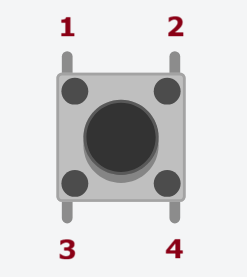
\includegraphics[width=0.5\linewidth]{Bryterposisjon.png}
	\caption{Bryter.}
	\label{fig:bryter}
\end{figure}
\section{Resultater}


\section{Diskusjon}

blah blah blah

\section{Konklusjon}

smrt smrt

referansebruk \cite{technical_name}

\begin{thebibliography}{9}
	\bibitem{technical_name}
	vet ikke hvordan dette funker.Vi bør gjøre dette så enkelt som mulig. 
\end{thebibliography}

\end{document}

